\section{EXPERIMENT}
A nominal goal of throwing a projectile 3.0m directly in front of the robot was chosen for testing purposes.  The estimated release point was set to the mean of the right arm's reachable area, 0.8m in $z$.  This resulted in a throwing velocity of 4.9m/s at $[\Theta, \Psi, \Phi] =[0.0^o,45.0^o, 3.8^o]$.  The projectile is a standard racquetball measuring 57mm in diameter and weighting 42.7g.

$L_d$ and the setup trajectory are created using the method shown in Section~\ref{sec:methodology} and following all specified constraints.  Fig.~\ref{fig:3dThrowPlot1} shows $L_d$ and the setup trajectory plotted within the SRM.

\begin{figure}[thpb]
  \centering
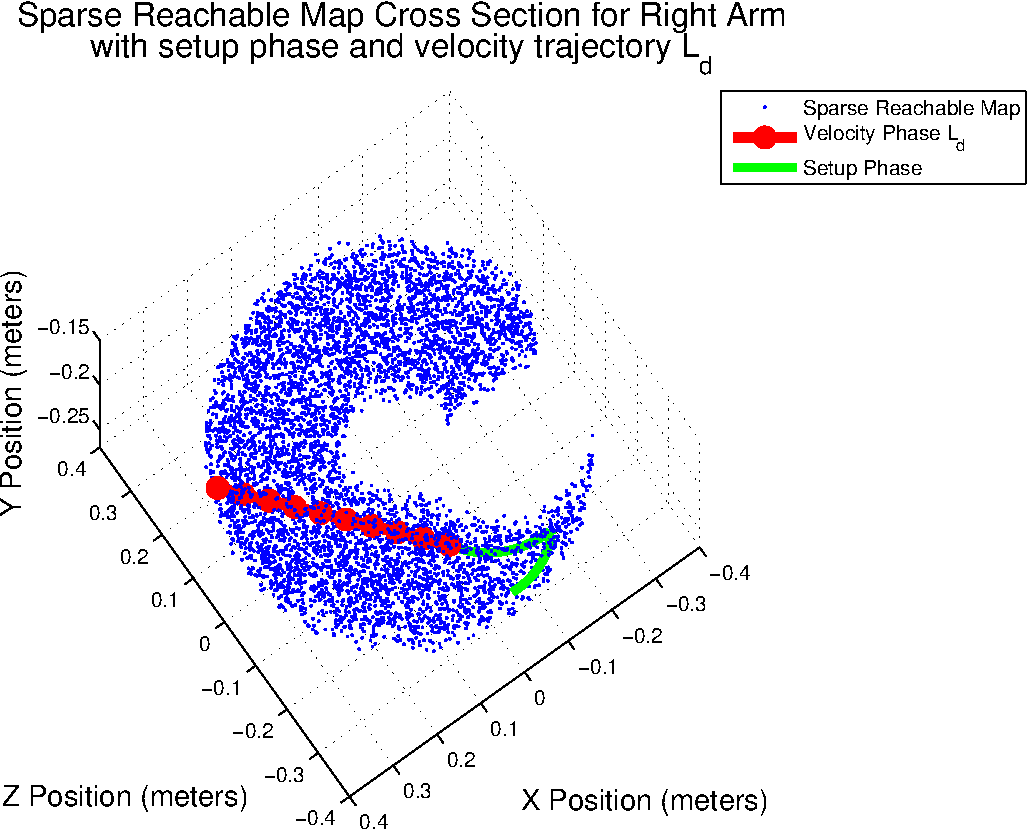
\includegraphics[width=1.0\columnwidth]{./MATLAB/throwTraj3D.pdf}
  \caption{Sparse Reachable Map Cross Section for Right Arm with setup phase and velocity trajectory $L_d$ }
  \label{fig:3dThrowPlot1}
\end{figure}


\begin{figure}[thpb]
  \centering
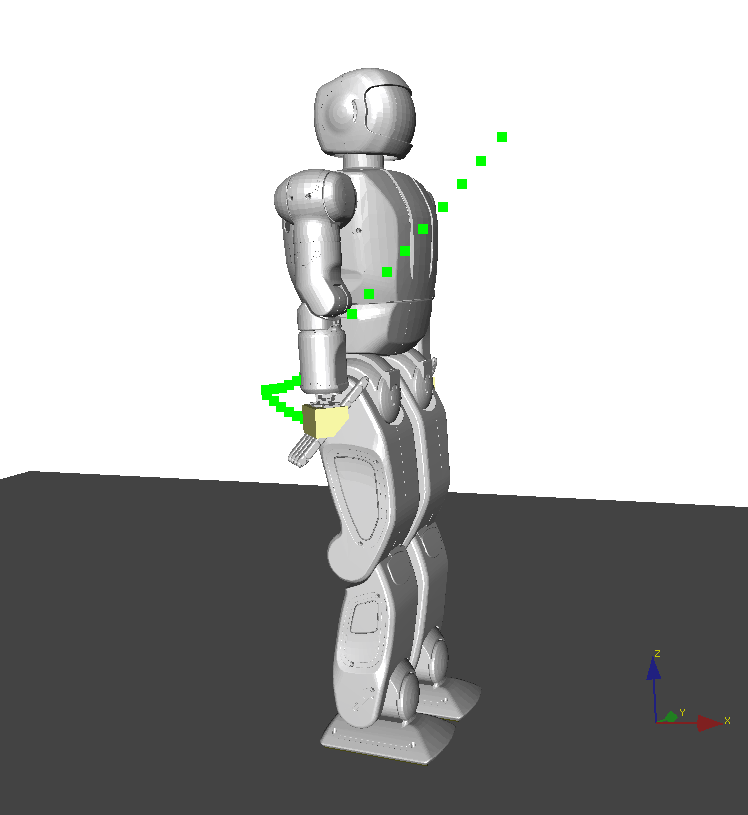
\includegraphics[width=0.25\columnwidth]{./pictures/ddFinal/vHside1.png}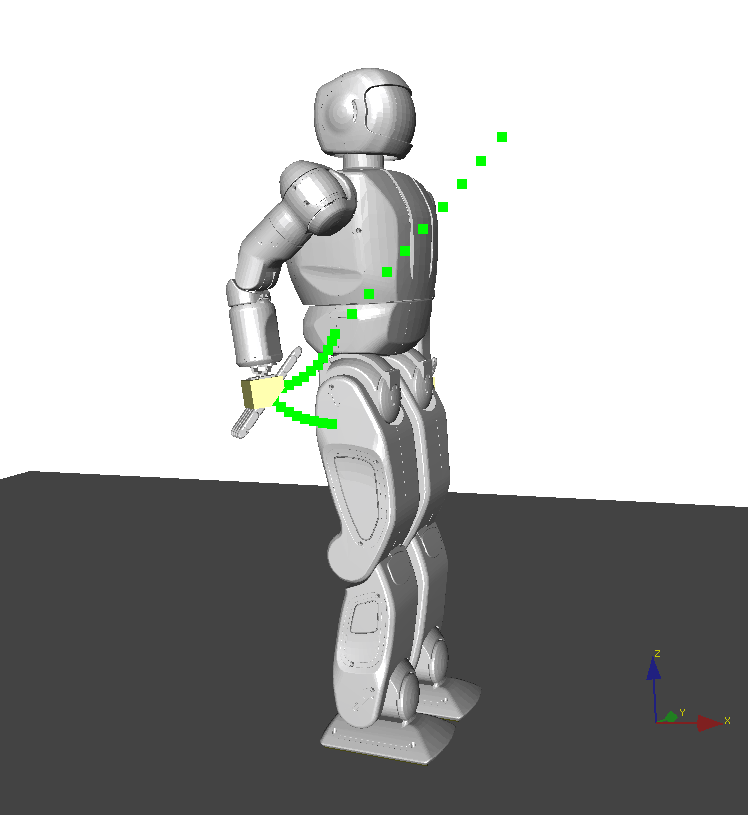
\includegraphics[width=0.25\columnwidth]{./pictures/ddFinal/vHside3.png}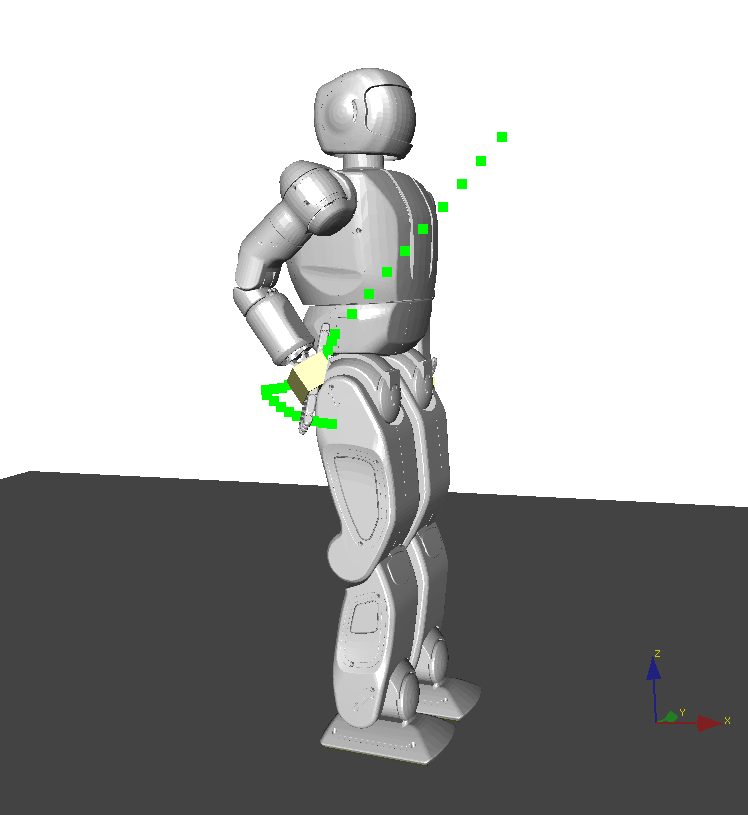
\includegraphics[width=0.25\columnwidth]{./pictures/ddFinal/vHside4.png}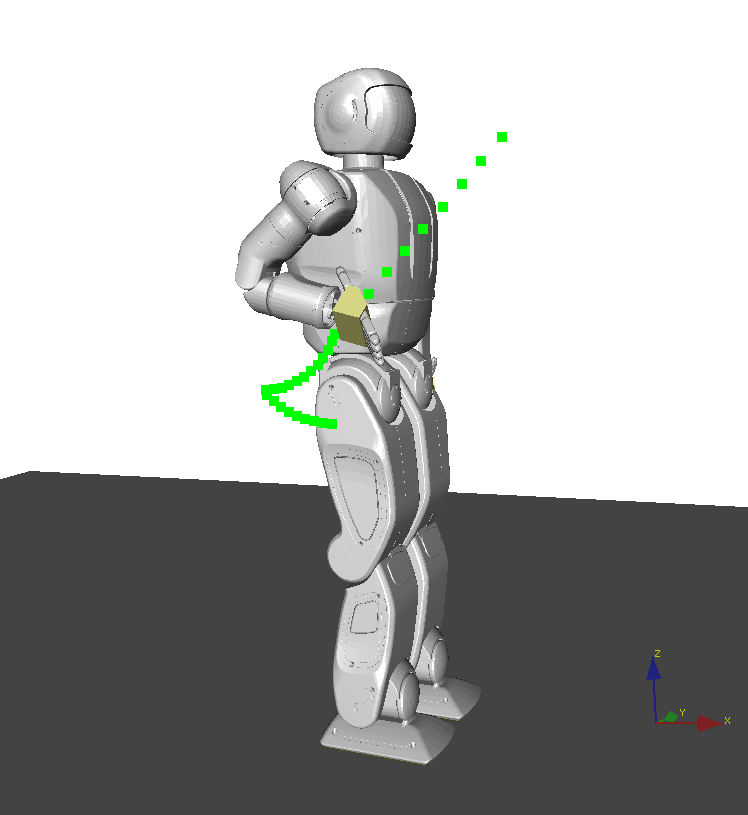
\includegraphics[width=0.25\columnwidth]{./pictures/ddFinal/vHside5.png}
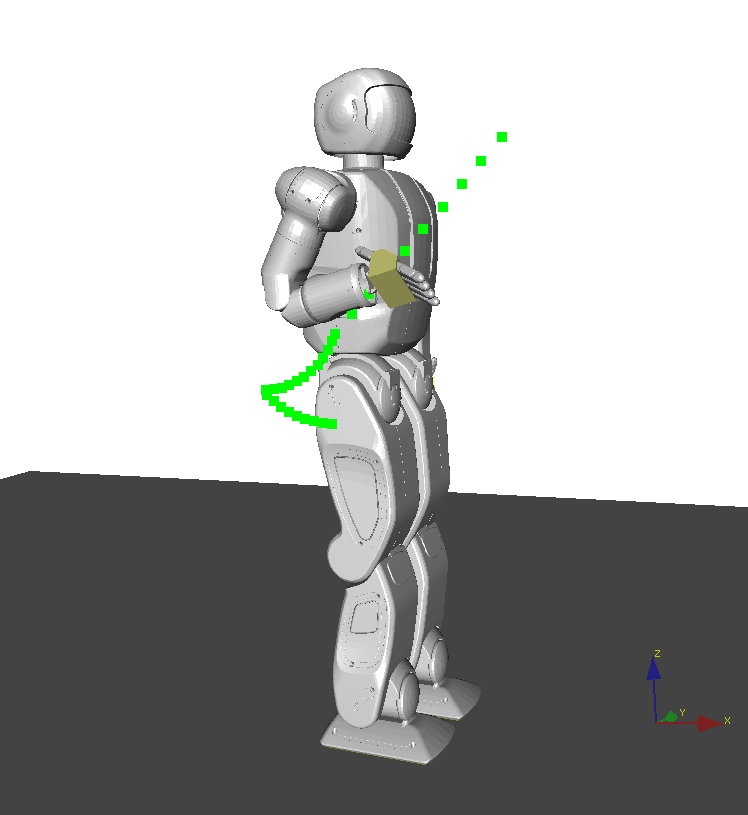
\includegraphics[width=0.25\columnwidth]{./pictures/ddFinal/vHside6.png}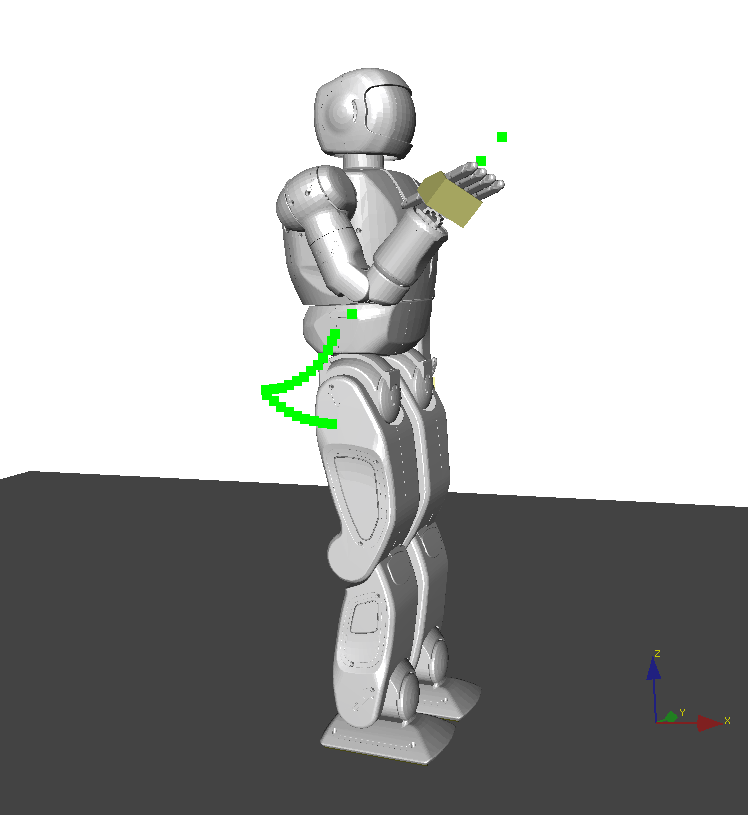
\includegraphics[width=0.25\columnwidth]{./pictures/ddFinal/vHside7.png}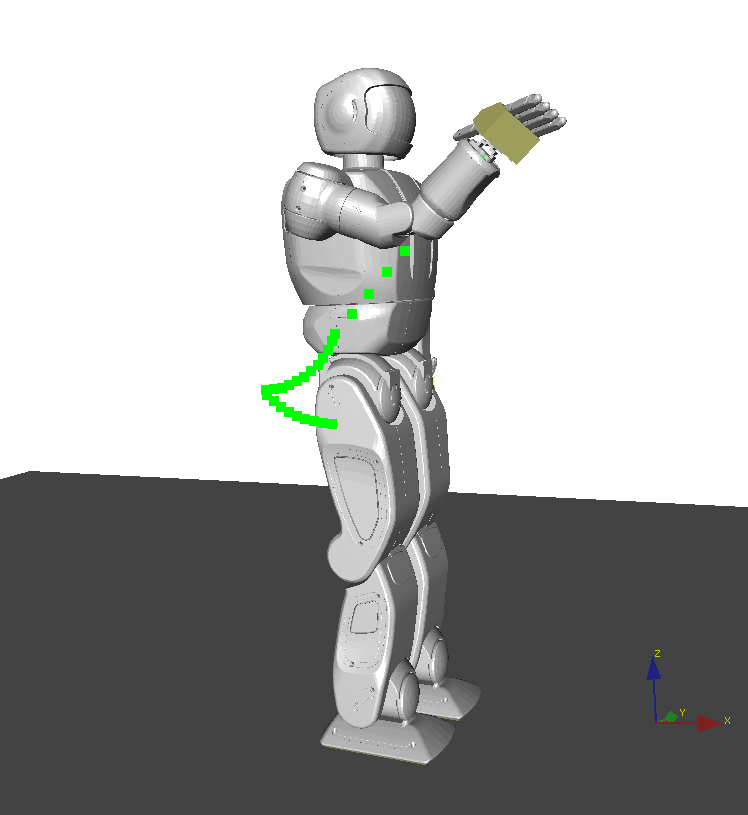
\includegraphics[width=0.25\columnwidth]{./pictures/ddFinal/vHside9.png}
  \caption{Jaemi Hubo running throwing trajectory $L_d$ immediately after the setup phase is completed.  $L_d(0)$ is top left.  Frames are read left to right and have a $\Delta t$ of 0.15s}
  \label{fig:fThrow}
\end{figure}



The trajectory was run on Jaemi Hubo with a position command period of 0.01s.  Fig~\ref{fig:3dThrowReal} shows the side profile of the Jaemi Hubo successfully running the trajectory.  The trajectory shown in Fig~\ref{fig:3dThrowReal} is considered an underhand throw, overhand and sidearm throws are also created with this method.

\begin{figure}[thpb]
  \centering
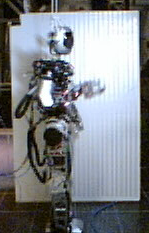
\includegraphics[width=0.25\columnwidth]{./pictures/slowMotion/1.png}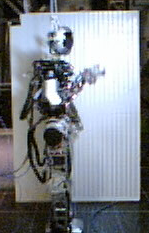
\includegraphics[width=0.25\columnwidth]{./pictures/slowMotion/2.png}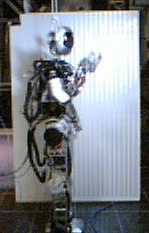
\includegraphics[width=0.25\columnwidth]{./pictures/slowMotion/3.png}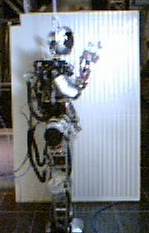
\includegraphics[width=0.25\columnwidth]{./pictures/slowMotion/4.png}
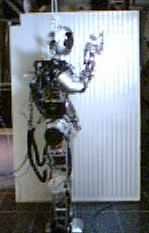
\includegraphics[width=0.25\columnwidth]{./pictures/slowMotion/5.png}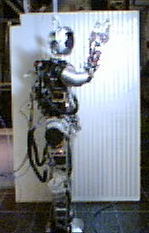
\includegraphics[width=0.25\columnwidth]{./pictures/slowMotion/6.png}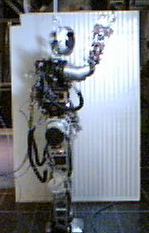
\includegraphics[width=0.25\columnwidth]{./pictures/slowMotion/7.png}
  \caption{Jaemi Hubo running throwing trajectory $L_d$ immediately after the setup phase is completed.  $L_d(0)$ is top left.  Frames are read left to right and have a $\Delta t$ of 0.15s}
  \label{fig:3dThrowReal}
\end{figure}

During the experiments the actual position of each joint was recorded.  The total time from the start of the setup phase to the end of the velocity phase is 0.31s.

